\documentclass[11pt]{article}

\usepackage[margin=1in]{geometry}
\usepackage{amsmath,amssymb,amsthm,mathtools}
\usepackage{booktabs}
\usepackage{tikz}
\usetikzlibrary{decorations.pathreplacing}

\newtheorem{theorem}{Theorem}
\newtheorem{lemma}{Lemma}
\newtheorem{remark}{Remark}

\DeclareMathOperator*{\argmax}{arg\,max}

\title{$\lambda$-Lower Bound Family}
\author{}
\date{}

\begin{document}

\maketitle

\section{Instance family}

We aim to find a lower bound on $\lambda$ by considering a more general family of instances of following form.

Our family of instances has $u$ many jobs of size $p$ which do not share a machine with any other job in $S_{OPT}$. The remaining machines all have a makespan of  $1$ in 
$S_{OPT}$ and have at least two jobs scheduled. $S_{WORST}$ results from $S_{OPT}$ by spreading the load of the $m-u$ machines with load $1$ to all machines resulting in load in $\frac{m-u}{m}$ on all machines. 
We then schedule the remaining $u$ jobs of size $p$ on top of this load.
The job size of all jobs that are are not of single scheduled jobs is determined such that there exists a schedule of these jobs in which exactly $m-u$ machines have load $1$ and there exists a schedule such that the load of all machines have exactly load $\frac{m-u}{m}$.        

\section{Job length determination}

We assume for this family of jobs that $u \geq 1$. 
We consider now only the set of instances of the above form for which $\frac{1}{k+1} \leq \frac{u}{m} \leq \frac{1}{k}$ with $k \geq 2$.
We define the job length of the jobs that are not single scheduled as follows. We have $m-u$ many jobs of size $1-\frac{u}{m}$ and $(k-1)u$ many jobs of size $\frac{u}{m}$.   
There remains a block of jobs of total size $(m-ku)\frac{u}{m}$. Which we now split with as little splitting steps as possible such that this load can be equally spread onto $u$ machines.
The load that we need for each machine in $S_{WORST}$ is $\frac{m-ku}{m}$. 
\begin{figure}[ht]
\centering

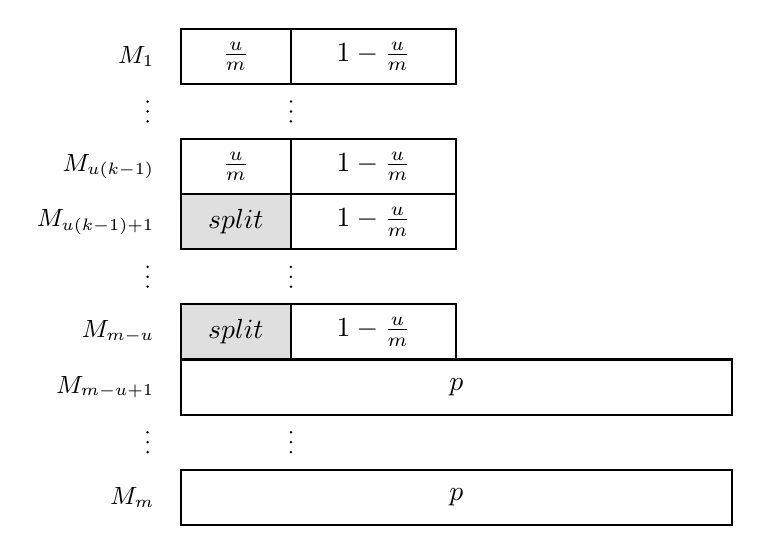
\begin{tikzpicture}[
    x=0.7cm,
    y=0.7cm,
    job/.style={
        draw,
        thick,
        fill=white,
        font=\small
    },
    machine/.style={font=\small}
]

% ------------------------------------------------
% Template idea:
% row      = displayed vertical row in the picture
% machine  = actual machine label shown on the left
%
% Use \machinerow{row}{machine label}
% Use \dotsrow{row}
% Use \jobblock{row}{start}{length}{job label}
% Use \jobblock[gray!25]{row}{start}{length}{job label} for shading
% ------------------------------------------------

\newcommand{\machinerow}[2]{
    \node[machine, anchor=east] at (-0.3,-#1+0.5) {$M_{#2}$};
}

\newcommand{\dotsrow}[1]{
    \foreach \dy in {-0.18,0,0.18} {
        \fill (-0.6,{-#1+0.5+\dy}) circle[radius=0.025];
        \fill (2,{-#1+0.5+\dy}) circle[radius=0.025];
    }
}

\newcommand{\jobblock}[5][white]{
    \draw[job, fill=#1] (#3,-#2) rectangle ++(#4,1);
    \node at ({#3 + #4/2},{-#2 + 0.5}) {$#5$};
}

% Displayed machine rows
\machinerow{1}{1}
\dotsrow{2}
\machinerow{3}{u(k-1)}
\machinerow{4}{u(k-1)+1}
\dotsrow{5}
\machinerow{6}{m-u}
\machinerow{7}{m-u+1}
\dotsrow{8}
\machinerow{9}{m}

% Example jobs
\jobblock{1}{0}{2}{\frac{u}{m}}
\jobblock{1}{2}{3}{1-\frac{u}{m}}

\jobblock{3}{0}{2}{\frac{u}{m}}
\jobblock{3}{2}{3}{1-\frac{u}{m}}

\jobblock[gray!25]{4}{0}{2}{split}
\jobblock{4}{2}{3}{1-\frac{u}{m}}

\jobblock[gray!25]{6}{0}{2}{split}
\jobblock{6}{2}{3}{1-\frac{u}{m}}
\jobblock{7}{0}{10}{p}
\jobblock{9}{0}{10}{p}

\end{tikzpicture}

\caption{Instance structure}
\label{fig:instance-structure}

\end{figure}
\subsection{Splitting}

Assume throughout that
\[
\gcd(m,u)=1
\]

The problem we are faced with is having \(N = m-ku\) unit lengths which we want to split using as few cuts as possible, so that they can be regrouped into \(u\) parts of equal total length.

Since \(0<N<u\), each of the \(u\) final parts must have total length
\[
\frac{N}{u}
=\frac{m-ku}{u}.
\]
Since \(\gcd(m,u)=1\), we also have
\[
\gcd(N,u)=1.
\]

\begin{figure}[h]
\centering
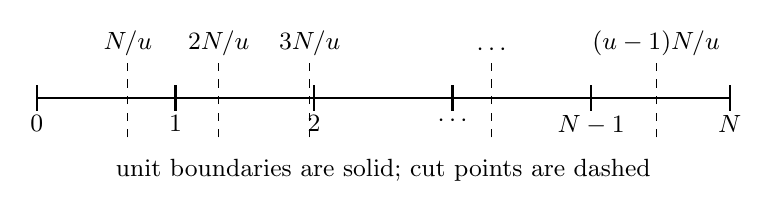
\begin{tikzpicture}[x=1.1cm,y=1cm]
  \draw[thick] (0,0) -- (8,0);
  \foreach \x/\lab in {0/0,1.6/1,3.2/2,4.8/{\cdots},6.4/{N-1},8/N} {
    \draw[thick] (\x,-0.16) -- (\x,0.16);
    \node[below,font=\small,fill=white,inner sep=1pt] at (\x,-0.18) {\(\lab\)};
  }

  \foreach \x/\lab in {1.05/{N/u},2.1/{2N/u},3.15/{3N/u},5.25/{\cdots},7.15/{(u-1)N/u}} {
    \draw[dashed] (\x,-0.5) -- (\x,0.5);
    \node[above,font=\small,fill=white,inner sep=1pt] at (\x,0.5) {\(\lab\)};
  }

  \node[below=0.65cm,font=\small] at (4,0) {unit boundaries are solid; cut points are dashed};
\end{tikzpicture}
\caption{The \(N=m-ku\) unit lengths are placed in one strip. The cuts divide the strip into \(u\) intervals of equal length \(N/u\).}
\end{figure}


\section*{Construction}

Line up the \(N=m-ku\) unit lengths into one block of total length \(N\). Make cuts at
\[
\frac{N}{u},\frac{2N}{u},\frac{3N}{u},\ldots,\frac{(u-1)N}{u}.
\]

The cut points divide the interval \([0,N]\) into \(u\) consecutive intervals
\[
I_j=\left[\frac{(j-1)N}{u},\frac{jN}{u}\right],
\qquad
j=1,2,\ldots,u.
\]
Each interval \(I_j\) has length \(N/u\), so each \(I_j\) is one of the desired final equal parts.
The unit pieces, however, have boundaries at the integers $0,1,2,\ldots,N$.
Since \(N<u\), each interval \(I_j\) has length less than \(1\). Therefore an interval \(I_j\) can contain at most one integer boundary in its interior.

If \(I_j\) contains no integer boundary, then it remains one physical piece of length
\[
\frac{N}{u}.
\]
If \(I_j\) contains an integer boundary \(i\), then that boundary splits \(I_j\) into two pieces.

\begin{figure}[h]
\centering
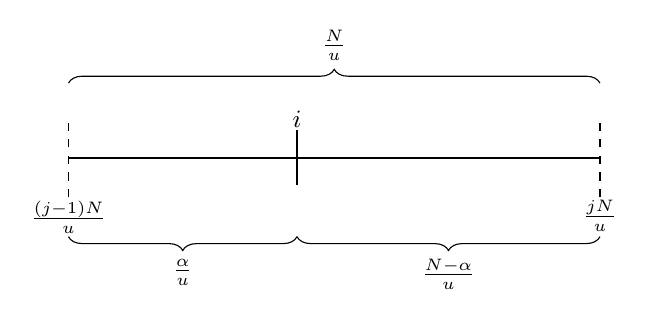
\begin{tikzpicture}[x=1.35cm,y=1cm]
  \draw[thick] (0,0) -- (5,0);
  \draw[dashed] (0,-0.5) -- (0,0.5);
  \draw[dashed] (5,-0.5) -- (5,0.5);
  \draw[thick] (2.15,-0.35) -- (2.15,0.35);

  \node[below,font=\small,fill=white,inner sep=1pt] at (0,-0.5) {\(\frac{(j-1)N}{u}\)};
  \node[below,font=\small,fill=white,inner sep=1pt] at (5,-0.5) {\(\frac{jN}{u}\)};
  \node[above,font=\small,fill=white,inner sep=1pt] at (2.15,0.35) {\(i\)};

  \draw[decorate,decoration={brace,mirror,amplitude=5pt}] (0,-1.0) -- (2.15,-1.0)
    node[midway,below=7pt,font=\small,fill=white,inner sep=1pt] {\(\frac{\alpha}{u}\)};
  \draw[decorate,decoration={brace,mirror,amplitude=5pt}] (2.15,-1.0) -- (5,-1.0)
    node[midway,below=7pt,font=\small,fill=white,inner sep=1pt] {\(\frac{N-\alpha}{u}\)};
  \draw[decorate,decoration={brace,amplitude=5pt}] (0,0.95) -- (5,0.95)
    node[midway,above=7pt,font=\small,fill=white,inner sep=1pt] {\(\frac{N}{u}\)};
\end{tikzpicture}
\caption{An equal interval \(I_j\) has length \(N/u<1\), so it contains at most one unit boundary. If it contains one, it is split into two lengths whose numerators add to \(N\).}
\end{figure}

There are \(N-1\) interior integer boundaries:
\[
1,2,\ldots,N-1.
\]
Thus \(N-1\) of the intervals \(I_j\) are split into two pieces, and the remaining
\[
u-(N-1)=u-N+1
\]
intervals are not split. Therefore there are $u-N+1$ many
pieces of length $\frac{N}{u}$.

It remains to identify the lengths created by the $N-1$ interior integer boundaries. Fix an integer boundary
\[
i\in\{1,2,\ldots,N-1\}.
\]
It lies in a unique interval \(I_j\), so
\[
\frac{(j-1)N}{u}<i<\frac{jN}{u}.
\]
The two pieces created around \(i\) have lengths
\[
i-\frac{(j-1)N}{u}
\]
and
\[
\frac{jN}{u}-i.
\]
Multiplying by \(u\), these lengths become
\[
iu-(j-1)N
\]
and
\[
jN-iu.
\]
These are positive integers whose sum is \(N\). Hence the two physical lengths are
\[
\frac{iu-(j-1)N}{u}
\qquad\text{and}\qquad
\frac{jN-iu}{u}.
\]
Now set
\[
\alpha=iu-(j-1)N.
\]
Then the second numerator is
\[
jN-iu=N-\alpha,
\]
because
\[
\bigl(iu-(j-1)N\bigr)+\bigl(jN-iu\bigr)=N.
\]
Thus the two physical lengths can be written as
\[
\frac{\alpha}{u}
\qquad\text{and}\qquad
\frac{N-\alpha}{u}
\]
for some \(\alpha\in\{1,2,\ldots,N-1\}\).

As \(i\) runs through \(1,2,\ldots,N-1\), the residues
\[
iu \pmod N
\]
run through all nonzero residues modulo \(N\), because \(\gcd(N,u)=1\). Therefore the values \(\alpha\) obtained are precisely
\[
1,2,\ldots,N-1,
\]
each once. Each such boundary contributes the pair
\[
\frac{\alpha}{u}
\quad\text{and}\quad
\frac{N-\alpha}{u}.
\]
Consequently every length
\[
\frac{1}{u},\frac{2}{u},\ldots,\frac{N-1}{u}
\]
appears exactly twice.

Combining this with the unsplit intervals gives the full list:
\[
2 \text{ pieces of length } \frac{1}{u},
\quad
2 \text{ pieces of length } \frac{2}{u},
\quad
\ldots,
\quad
2 \text{ pieces of length } \frac{N-1}{u},
\]
and
\[
u-N+1 \text{ pieces of length } \frac{N}{u}.
\]


For the family of instaces introducedm we do not deal with unit length intervals that need to be split but intervals of length $\frac{u}{m}$. 
Scaling all pieces by $\frac{u}{m}$, we get the following list of pieces:

\[
2 \text{ pieces of length } \frac{1}{m},
\quad
2 \text{ pieces of length } \frac{2}{m},
\quad
\ldots, 
\quad
2 \text{ pieces of length } \frac{m-ku-1}{m},
\]
and

\[
u-(m-ku)+1=((k+1)u-m+1) \text{ pieces of length } \frac{m-ku}{m}.
\]

\section{Optimzation}

We now can write down $\lambda$ for the family of instances introduced above. Let \(m\) be the number of machines, and let \(u\) be the number of jobs of size \(p\) that are single scheduled in \(S_{OPT}\). Assume  
$ 0 \leq \alpha \leq \frac12$


We want to maximize
\[
\lambda(m,u,p)=\frac{
(m-u)\left(1-\frac um\right)^2
 +u\left(p+1-\frac um\right)^2
 +(2\alpha-1)B
}{
(m-u)+up^2+(2\alpha-1)B
},
\]
where
\[
\begin{aligned}
B&=\sum_{j=1}^{m-ku-1}2\left(\frac{j}{m}\right)^2+\left((k+1)u-m+1\right)\left(\frac{m-ku}{m}\right)^2
+up^2
+(m-u)\left(1-\frac um\right)^2
+(k-1)\frac{u^3}{m^2}\\
&=\frac{(m-ku-1)(m-ku)(2m-2ku-1)}{3m^2}  \\
&+\left((k+1)u-m+1\right)\left(\frac{m-ku}{m}\right)^2
+up^2
+(m-u)\left(1-\frac um\right)^2
+(k-1)\frac{u^3}{m^2}.
\end{aligned}
\]

\subsection{Normalization}

Set
\[
        x=\frac{u}{m}, \qquad r=1-kx=\frac{m-ku}{m}.
\]
The constraint becomes
\[
        \frac{1}{k+1}\leq x\leq \frac1k,
        \qquad 0\leq r\leq \frac{1}{k+1}.
\]
Also set
\[
        b=1-2\alpha.
\]
Then \(0\leq b\leq 1\), and
\[
        2\alpha-1=-b.
\]

We first separate the \(p^2\)-term in B. Write
\[
        B=mxp^2+R,
\]
where
\[
\begin{aligned}
R={}&
\frac{(m-ku-1)(m-ku)(2m-2ku-1)}{3m^2}  \\
&+\left((k+1)u-m+1\right)\left(\frac{m-ku}{m}\right)^2
+(m-u)\left(1-\frac um\right)^2
+(k-1)\frac{u^3}{m^2}.
\end{aligned}
\]

Since \(m-ku=mr\), the first term satisfies
\[
\begin{aligned}
\frac{(m-ku-1)(m-ku)(2m-2ku-1)}{3m^2}
&=
\frac{(mr-1)(mr)(2mr-1)}{3m^2}.
\end{aligned}
\]
Dividing by \(m\),
\[
\begin{aligned}
\frac{(mr-1)(mr)(2mr-1)}{3m^3}
&=
\frac{2r^3}{3}-\frac{r^2}{m}+\frac{r}{3m^2}.
\end{aligned}
\]
The second term gives
\[
\begin{aligned}
\frac{1}{m}
\left((k+1)u-m+1\right)\left(\frac{m-ku}{m}\right)^2
&=
\left((k+1)x-1+\frac1m\right)r^2.
\end{aligned}
\]
Using \(1=kx+r\), we have
\[
        (k+1)x-1=x-r.
\]
Therefore
\[
\begin{aligned}
\frac{R}{m}
&=
\left(\frac{2r^3}{3}-\frac{r^2}{m}+\frac{r}{3m^2}\right)
+
\left(x-r+\frac1m\right)r^2
+(1-x)^3
+(k-1)x^3 \\
&=
\frac{2r^3}{3}-\frac{r^2}{m}+\frac{r}{3m^2}
+xr^2-r^3+\frac{r^2}{m}
+(1-x)^3
+(k-1)x^3 \\
&=
xr^2-\frac{r^3}{3}
+(1-x)^3
+(k-1)x^3
+\frac{r}{3m^2}.
\end{aligned}
\]
Which we name:
\[
        \rho(x,m)
        =
        \frac{R}{m}
        =
        xr^2-\frac{r^3}{3}
        +(1-x)^3
        +(k-1)x^3
        +\frac{r}{3m^2}.
\]

Simplifying the numerator and denominator of \(\lambda\) gives

\[
\begin{aligned}
N-D
={}&
(m-u)\left(1-\frac um\right)^2
+u\left(p+1-\frac um\right)^2
-(m-u)-up^2.
\end{aligned}
\]
Substituting \(x=u/m\), this becomes
\[
\begin{aligned}
N-D
&=
m(1-x)^3
 +mx\bigl(p+1-x\bigr)^2
 -m(1-x)-mxp^2 \\
&=
m(1-x)^3
 +mx\left(p^2+2p(1-x)+(1-x)^2\right)
 -m(1-x)-mxp^2 \\
&=
m(1-x)\left((1-x)-1+2xp\right) \\
&=
mx(1-x)(2p-1).
\end{aligned}
\]
Thus
\[
        \lambda(x,m,p)=1+\frac{mx(1-x)(2p-1)}{D}.
\]

The denominator is
\[
\begin{aligned}
D
&=
m(1-x)+mxp^2-b(mx p^2+R) \\
&=
m(1-x)+mxp^2-bmxp^2-bR \\
&=
m(1-x)+2\alpha mxp^2-bR \\
&=
m\left(2\alpha xp^2+(1-x)-b\rho(x,m)\right).
\end{aligned}
\]
Define
\[
        c(x,m,\alpha)=(1-x)-(1-2\alpha)\rho(x,m).
\]
Then, for \(\alpha>0\),
\[
        \lambda(x,m,p)
        =
        1+
        \frac{x(1-x)(2p-1)}{2\alpha xp^2+c(x,m,\alpha)}.
\]

\subsection{Maximizing in \(p\)}

For fixed \(x,m,\alpha\), define
\[
        c=c(x,m,\alpha).
\]
Then
\[
        \lambda(x,m,p)
        =
        1+
        \frac{x(1-x)(2p-1)}{2\alpha xp^2+c}.
\]
Equivalently,
\[
        \lambda(x,m,p)
        =
        1+
        \frac{1-x}{2\alpha}
        \frac{2p-1}{p^2+q},
        \qquad
        q=\frac{c}{2\alpha x}.
\]
Differentiate the \(p\)-dependent factor:
\[
\begin{aligned}
\frac{d}{dp}\left(\frac{2p-1}{p^2+q}\right)
&=
\frac{2(p^2+q)-(2p-1)(2p)}{(p^2+q)^2} \\
&=
\frac{-2p^2+2p+2q}{(p^2+q)^2}.
\end{aligned}
\]
The critical point is therefore determined by
\[
        p^2-p-q=0.
\]
Since \(p>0\), the maximizing critical point is
\[
        p^*
        =
        \frac{1+\sqrt{1+4q}}{2}
        =
        \frac{1+\sqrt{1+\frac{2c}{\alpha x}}}{2}.
\]
At this point,
\[
        q=(p^*)^2-p^*,
\]
so
\[
\begin{aligned}
\frac{2p^*-1}{(p^*)^2+q}
&=
\frac{2p^*-1}{(p^*)^2+(p^*)^2-p^*}  \\
&=
\frac{2p^*-1}{p^*(2p^*-1)} \\
&=
\frac{1}{p^*}.
\end{aligned}
\]
Hence the optimized value at fixed \(x,m\) is
\[
\boxed{
        \lambda^*(x,m)
        =
        1+
        \frac{1-x}{2\alpha p^*}
        =
        1+
        \frac{1-x}{\alpha\left(1+\sqrt{1+\frac{2c(x,m,\alpha)}{\alpha x}}\right)}
        }.
\]

\subsection{Maximizing in \(x\) and \(m\)}


We first argue, that after optimizing over \(p\), the best value is
obtained at one of the two endpoints
\[
        x=\frac{1}{k+1}
        \qquad\text{or}\qquad
        x=\frac1k.
\]

We set
\[
        n=m-ku.
\]
The constraint
\[
        \frac{1}{k+1}\leq \frac{u}{m}\leq \frac1k
\]
is equivalent to
\[
        0\leq n\leq u.
\]
So that we can write: 
\[
        t=\frac{n}{u},
        \qquad 0\leq t\leq 1.
\]
Since
\[
        m=ku+n=u(k+t),
\]
we get
\[
        x=\frac{u}{m}=\frac{1}{k+t},
        \qquad
        r=1-kx=\frac{t}{k+t}.
\]
Thus the upper endpoint \(x=1/k\) corresponds to \(t=0\), and the lower
endpoint \(x=1/(k+1)\) corresponds to \(t=1\).

Using the formula for \(\rho(x,m)\), we obtain
\[
\begin{aligned}
\rho(t,u)
&=
xr^2-\frac{r^3}{3}
 +(1-x)^3
 +(k-1)x^3
 +\frac{r}{3m^2} \\
&=
\frac{1}{(k+t)^3}
\left[
t^2-\frac{t^3}{3}
 +(k+t-1)^3
 +(k-1)
 +\frac{t}{3u^2}
\right].
\end{aligned}
\]
Define
\[
        s=k+t,
\]
and
\[
        A_u(t)
        =
        t^2-\frac{t^3}{3}
        +(k+t-1)^3
        +(k-1)
        +\frac{t}{3u^2}.
\]
Then
\[
        \rho(t,u)=\frac{A_u(t)}{s^3}.
\]
Also
\[
        1-x=\frac{s-1}{s},
        \qquad
        \frac{c(x,m,\alpha)}{x}
        =
        s-1-(1-2\alpha)\frac{A_u(t)}{s^2}.
\]
Therefore the optimized value can be written as
\[
        \lambda^*(t,u)
        =
        1+
        \frac{s-1}{
        \alpha s\left(
        1+\sqrt{
        1+\frac{2}{\alpha}
        \left(
        s-1-(1-2\alpha)\frac{A_u(t)}{s^2}
        \right)
        }
        \right)
        }.
\]

For fixed \(t\), the only dependence on \(u\) is through the term
\[
        \frac{t}{3u^2}
\]
inside \(A_u(t)\). Since \(1-2\alpha\geq 0\), increasing \(A_u(t)\) decreases
\[
        s-1-(1-2\alpha)\frac{A_u(t)}{s^2},
\]
and therefore decreases the square root in the denominator of \(F^*(t,u)\).
Thus \(F^*(t,u)\) is increasing in \(A_u(t)\). Hence, for fixed \(t\),
the largest possible value is obtained by taking the smallest admissible
\(u\).

In particular, for every admissible integer pair \((m,u)\),
For every admissible integer pair \((m,u)\),
\[
        F^*(t,u)\leq \overline F(t),
\]
where \(s=k+t\) and
\[
        \overline F(t)
        =
        1+
        \frac{s-1}{
        \alpha s\left(
        1+\sqrt{
        1+\frac{2}{\alpha}
        \left(
        s-1-(1-2\alpha)\frac{\overline A(t)}{s^2}
        \right)
        }
        \right)
        },
\]
and
\[
        \overline A(t)
        =
        t^2-\frac{t^3}{3}
        +(k+t-1)^3
        +(k-1)
        +\frac{t}{3}.
\]
This upper envelope is obtained by putting \(u=1\). Although \(u=1\) is
compatible with the original integer problem only at \(t=0\) and \(t=1\),
it gives a convenient upper bound for all \(0\leq t\leq 1\).

We claim that \(\overline F\) has no interior maximum on \([0,1]\).

\begin{lemma}
Assume
\[
        k\geq 2,\qquad 0<\alpha\leq \frac12.
\]
Every critical point of \(\overline F\) in \((0,1)\) is a strict local
minimum.
\end{lemma}

\begin{proof}
First,
\[
        \overline A'(t)
        =
        2t-t^2+3(k+t-1)^2+\frac13.
\]
Let \(t\in(0,1)\) be a critical point of \(\overline F\). A direct
differentiation, followed by substitution of the critical-point equation
\(\overline F'(t)=0\), gives
\[
        \overline F''(t)
        =
        \frac{
        (1-2\alpha)Q_{k,\alpha}(t)
        }{
        \alpha^2s^3(s-1)
        \left(
        1+\frac{2}{\alpha}
        \left(
        s-1-(1-2\alpha)\frac{\overline A(t)}{s^2}
        \right)
        \right)^{3/2}
        },
\]
where
\[
\begin{aligned}
Q_{k,\alpha}(t)
={}&
\frac{\alpha^2}{3s^2}
\left[
3(k-1)^2+6(k-1)t+2t^2+1
\right]^2                                      \\
&+
\frac{2\alpha}{s}
\left[
3(k-1)^2+6(k-1)t+2t^2+1
\right]                                      \\
&+
\frac{2\alpha}{s}
(1-t)\left(3(k-1)+2t\right).
\end{aligned}
\]
For
\[
        k\geq 2,\qquad 0<\alpha\leq \frac12,\qquad 0<t<1,
\]
the denominator is positive: indeed \(\alpha>0\), \(s=k+t>1\), and the
quantity under the square root is positive because \(\overline F(t)\) is
real-valued on the interval under consideration. Also \(1-2\alpha\geq 0\), and
every term in \(Q_{k,\alpha}(t)\) is nonnegative. Moreover,
\[
        3(k-1)^2+6(k-1)t+2t^2+1>0,
\]
so \(Q_{k,\alpha}(t)>0\). Hence
\[
        \overline F''(t)>0.
\]
Thus every interior critical point is a strict local minimum.
\end{proof}

Therefore \(\overline F\) has no interior local maximum. Since
\(\overline F\) is continuous on \([0,1]\), its maximum is attained at an
endpoint:
\[
        \overline F(t)
        \leq
        \max\{\overline F(0),\overline F(1)\}
        \qquad (0\leq t\leq 1).
\]
Finally, because \(F^*(t,u)\leq \overline F(t)\), the original integer
problem is also maximized at one of the two endpoints,
\[
        t=0
        \qquad\text{or}\qquad
        t=1.
\]

\section{Maximum at the endpoints}

The remaining maximization is over integer pairs \((m,u)\) satisfying
\[
        \frac{1}{k+1}\leq \frac um\leq \frac1k.
\]
The maximum is attained at one of the two boundary ratios:
\[
        \frac um=\frac{1}{k+1}
        \qquad\text{or}\qquad
        \frac um=\frac1k.
\]
The corresponding integer maximizers are
\[
        (m,u)=(k+1,1)
        \qquad\text{and}\qquad
        (m,u)=(k,1).
\]

\subsection{\(x=\frac{1}{k+1}\)}

Take
\[
        m=k+1,\qquad u=1,\qquad x=\frac{1}{k+1}.
\]
And simply evaluate the formulas at this point. We have
\[
        r=1-kx=\frac{1}{k+1}.
\]
Using the formula for \(\rho\),
\[
\begin{aligned}
\rho_L
&=
xr^2-\frac{r^3}{3}
 +(1-x)^3
 +(k-1)x^3
 +\frac{r}{3m^2} \\
&=
\frac{k^3+k}{(k+1)^3} \\
&=
\frac{k(k^2+1)}{(k+1)^3}.
\end{aligned}
\]
$\rho_L$ denoting the value of \(\rho\) at the lower endpoint \(x=1/(k+1)\).
Thus
\[
\begin{aligned}
c_L
&=
1-\frac{1}{k+1}
-(1-2\alpha)\frac{k(k^2+1)}{(k+1)^3} \\
&=
\frac{2k\left(k+\alpha(k^2+1)\right)}{(k+1)^3}.
\end{aligned}
\]
Therefore
\[
\frac{2c_L}{\alpha x}
=
\frac{2c_L}{\alpha/(k+1)}
=
\frac{4k\left(k+\alpha(k^2+1)\right)}{\alpha(k+1)^2}.
\]
So the optimizing \(p\) on the lower branch is
\[
\boxed{
p_L
=
\frac{
1+\sqrt{
1+\frac{4k\left(k+\alpha(k^2+1)\right)}{\alpha(k+1)^2}
}
}{2}
}.
\]
The corresponding value is
\[
\boxed{
L_k(\alpha)
=
1+
\frac{k}{
\alpha(k+1)\left(
1+\sqrt{
1+\frac{4k\left(k+\alpha(k^2+1)\right)}{\alpha(k+1)^2}
}
\right)}
}.
\]

\subsection{\(x=\frac{1}{k}\)}

Take
\[
        m=k,\qquad u=1,\qquad x=\frac1k.
\]
Then
\[
        r=1-kx=0.
\]
So simillarly to the previous case, we can evaluate \(\rho\) at this point:
\[
\begin{aligned}
\rho_U
&=
(1-x)^3+(k-1)x^3 \\
&=
\frac{(k-1)\left((k-1)^2+1\right)}{k^3}.
\end{aligned}
\]
Thus
\[
\begin{aligned}
c_U
&=
1-\frac1k
-(1-2\alpha)
\frac{(k-1)\left((k-1)^2+1\right)}{k^3} \\
&=
\frac{
2(k-1)^2
 +2\alpha(k-1)\left((k-1)^2+1\right)
}{k^3} \\
&=
\frac{
2(k-1)\left((k-1)+\alpha\left((k-1)^2+1\right)\right)
}{k^3}.
\end{aligned}
\]
Equivalently,
\[
        (k-1)^2+1=k^2-2k+2.
\]
Hence
\[
\frac{2c_U}{\alpha x}
=
\frac{2c_U}{\alpha/k}
=
\frac{
4(k-1)\left((k-1)+\alpha(k^2-2k+2)\right)
}{\alpha k^2}.
\]
The optimizing \(p\) on the upper branch is
\[
\boxed{
p_U
=
\frac{
1+\sqrt{
1+
\frac{
4(k-1)\left((k-1)+\alpha(k^2-2k+2)\right)
}{\alpha k^2}
}
}{2}
}.
\]
The corresponding value is
\[
\boxed{
U_k(\alpha)
=
1+
\frac{k-1}{
\alpha k\left(
1+\sqrt{
1+
\frac{
4(k-1)\left((k-1)+\alpha(k^2-2k+2)\right)
}{\alpha k^2}
}
\right)}
}.
\]

\section{Comparison of the Cases}

For \(0<\alpha\leq 1/2\), the maximum is
\[
        \max\{L_k(\alpha),U_k(\alpha)\}.
\]
The switching point is obtained by solving
\[
        L_k(\alpha)=U_k(\alpha).
\]
After substituting the displayed formulas for \(L_k(\alpha)\) and \(U_k(\alpha)\), isolating one square-root term, and squaring, the equality reduces to the linear equation
\[
        1-\alpha\left(k^4-2k^3-2k^2+k+3\right)=0.
\]
Therefore the formal switching value is
\[
\boxed{
        \alpha_k=
        \frac{1}{k^4-2k^3-2k^2+k+3}
        }.
\]

For \(k=2\), the denominator is
\[
        2^4-2\cdot 2^3-2\cdot 2^2+2+3
        =
        -3,
\]
so there is no positive switching point. In this case \(L_2(\alpha)>U_2(\alpha)\) for every
\[
        0<\alpha\leq \frac12.
\]

For \(k\geq 3\), the denominator is positive and gives a genuine switching point. Thus
\[
        L_k(\alpha)>U_k(\alpha)
        \quad\Longleftrightarrow\quad
        0<\alpha<\alpha_k,
\]
and
\[
        U_k(\alpha)>L_k(\alpha)
        \quad\Longleftrightarrow\quad
        \alpha_k<\alpha\leq \frac12.
\]
At \(\alpha=\alpha_k\), both branches give the same value.

\subsection{\(\alpha=0\)}

When \(\alpha=0\), we have \(2\alpha-1=-1\). The \(up^2\)-term in the denominator cancels against the \(up^2\)-term inside \(\mathcal B\):
\[
        up^2-(up^2)=0.
\]
The numerator still contains the term
\[
        u\left(p+1-\frac um\right)^2-up^2
        =
        2u\left(1-\frac um\right)p
        +u\left(1-\frac um\right)^2,
\]
which grows linearly in \(p\). Hence, as \(p\to\infty\), the ratio is unbounded above.

Therefore,
\[
\boxed{
        \alpha=0
        \quad\Longrightarrow\quad
        \sup F=+\infty.
        }
\]

\section{Maximum}

For \(\alpha=0\), the objective is unbounded above.

For \(0<\alpha\leq 1/2\), define
\[
\boxed{
L_k(\alpha)
=
1+
\frac{k}{
\alpha(k+1)\left(
1+\sqrt{
1+\frac{4k\left(k+\alpha(k^2+1)\right)}{\alpha(k+1)^2}
}
\right)}
}
\]
and
\[
\boxed{
U_k(\alpha)
=
1+
\frac{k-1}{
\alpha k\left(
1+\sqrt{
1+
\frac{
4(k-1)\left((k-1)+\alpha(k^2-2k+2)\right)
}{\alpha k^2}
}
\right)}
}.
\]
Then
\[
\boxed{
        \max F=\max\{L_k(\alpha),U_k(\alpha)\}.
        }
\]

More explicitly:

\[
\boxed{
\begin{array}{ll}
k=2,\ 0<\alpha\leq \frac12:
&
\max F=L_2(\alpha),
\quad (m,u)=(3,1),
\quad p=p_L.
\end{array}
}
\]

For \(k\geq 3\), let
\[
        \alpha_k=
        \frac{1}{k^4-2k^3-2k^2+k+3}.
\]
Then
\[
\boxed{
\begin{array}{lll}
0<\alpha<\alpha_k:
&
\max F=L_k(\alpha),
&
(m,u)=(k+1,1),\ p=p_L,
\\[6pt]
\alpha=\alpha_k:
&
\max F=L_k(\alpha)=U_k(\alpha),
&
(m,u)=(k+1,1)\text{ or }(k,1),
\\[6pt]
\alpha_k<\alpha\leq \frac12:
&
\max F=U_k(\alpha),
&
(m,u)=(k,1),\ p=p_U.
\end{array}
}
\]

Here
\[
\boxed{
p_L
=
\frac{
1+\sqrt{
1+\frac{4k\left(k+\alpha(k^2+1)\right)}{\alpha(k+1)^2}
}
}{2}
}
\]
and
\[
\boxed{
p_U
=
\frac{
1+\sqrt{
1+
\frac{
4(k-1)\left((k-1)+\alpha(k^2-2k+2)\right)
}{\alpha k^2}
}
}{2}
}.
\]

\end{document}
